\def\year{2024}\relax
%File: formatting-instructions-latex-2022.tex
%release 2022.1
\documentclass[letterpaper]{article} % DO NOT CHANGE THIS
\usepackage[submission]{aaai24}  % DO NOT CHANGE THIS
% \usepackage[submission]{aaai24}  % DO NOT CHANGE THIS
\usepackage{times}  % DO NOT CHANGE THIS
\usepackage{helvet}  % DO NOT CHANGE THIS
\usepackage{courier}  % DO NOT CHANGE THIS
\usepackage[hyphens]{url}  % DO NOT CHANGE THIS
\usepackage{graphicx} % DO NOT CHANGE THIS
\urlstyle{rm} % DO NOT CHANGE THIS
\def\UrlFont{\rm}  % DO NOT CHANGE THIS
\usepackage{natbib}  % DO NOT CHANGE THIS AND DO NOT ADD ANY OPTIONS TO IT
\usepackage{caption} % DO NOT CHANGE THIS AND DO NOT ADD ANY OPTIONS TO IT
\frenchspacing  % DO NOT CHANGE THIS
\setlength{\pdfpagewidth}{8.5in} % DO NOT CHANGE THIS
\setlength{\pdfpageheight}{11in} % DO NOT CHANGE THIS

%
% These are recommended to typeset algorithms but not required. See the subsubsection on algorithms. Remove them if you don't have algorithms in your paper.
\usepackage{algorithm}
\usepackage{algorithmic}


%%%%%%%%%%%%%%% US %%%%%%%%%%%%%%%%%
%  for beautifying tables
\usepackage{booktabs}
% Package tabularx provides the automatic adaption of cell width of cells specified with X type.
\usepackage{tabularx}

% just makes the table prettier (see \toprule, \bottomrule, etc. commands below)
\usepackage{booktabs}
\usepackage{multirow}
\usepackage{color}
\usepackage{xcolor}
\usepackage{colortbl}
% \usepackage{balance}

\usepackage{siunitx}

\usepackage{mathtools}

%%%%%%%%%%%%%%% US %%%%%%%%%%%%%%%%%

%
% These are recommended to typeset listings but not required. See the subsubsection on listing. Remove this block if you don't have listings in your paper.
\usepackage{newfloat}
\usepackage{listings}
\DeclareCaptionStyle{ruled}{labelfont=normalfont,labelsep=colon,strut=off} % DO NOT CHANGE THIS
\lstset{%
	basicstyle={\footnotesize\ttfamily},% footnotesize acceptable for monospace
	numbers=left,numberstyle=\footnotesize,xleftmargin=2em,% show line numbers, remove this entire line if you don't want the numbers.
	aboveskip=0pt,belowskip=0pt,%
	showstringspaces=false,tabsize=2,breaklines=true}
\floatstyle{ruled}
\newfloat{listing}{tb}{lst}{}
\floatname{listing}{Listing}


% ---------------------------
%  for tick boxes - error analysis
% \usepackage{graphicx}
% \usepackage{array}
% \usepackage{pifont}
% \usepackage{amssymb}
% \usepackage{adjustbox}
\usepackage{graphicx}
\usepackage{amssymb} % for the checkmark and crossmark symbols
\usepackage{adjustbox} % for adjusting the symbols

% ---------------------------
\usepackage{multicol}
% for multicolumn code
% ---------------------------
%
%\nocopyright
%
% Keep the \pdfinfo as shown here. There's no need
% for you to add the /Title and /Author tags.
\pdfinfo{
/TemplateVersion (2024.1)
}

% DISALLOWED PACKAGES
% \usepackage{authblk} -- This package is specifically forbidden
% \usepackage{balance} -- This package is specifically forbidden
% \usepackage{color (if used in text)
% \usepackage{CJK} -- This package is specifically forbidden
% \usepackage{float} -- This package is specifically forbidden
% \usepackage{flushend} -- This package is specifically forbidden
% \usepackage{fontenc} -- This package is specifically forbidden
% \usepackage{fullpage} -- This package is specifically forbidden
% \usepackage{geometry} -- This package is specifically forbidden
% \usepackage{grffile} -- This package is specifically forbidden
% \usepackage{hyperref} -- This package is specifically forbidden
% \usepackage{navigator} -- This package is specifically forbidden
% (or any other package that embeds links such as navigator or hyperref)
% \indentfirst} -- This package is specifically forbidden
% \layout} -- This package is specifically forbidden
% \multicol} -- This package is specifically forbidden
% \nameref} -- This package is specifically forbidden
% \usepackage{savetrees} -- This package is specifically forbidden
% \usepackage{setspace} -- This package is specifically forbidden
% \usepackage{stfloats} -- This package is specifically forbidden
% \usepackage{tabu} -- This package is specifically forbidden
% \usepackage{titlesec} -- This package is specifically forbidden
% \usepackage{tocbibind} -- This package is specifically forbidden
% \usepackage{ulem} -- This package is specifically forbidden
% \usepackage{wrapfig} -- This package is specifically forbidden
% DISALLOWED COMMANDS
% \nocopyright -- Your paper will not be published if you use this command
% \addtolength -- This command may not be used
% \balance -- This command may not be used
% \baselinestretch -- Your paper will not be published if you use this command
% \clearpage -- No page breaks of any kind may be used for the final version of your paper
% \columnsep -- This command may not be used
% \newpage -- No page breaks of any kind may be used for the final version of your paper
% \pagebreak -- No page breaks of any kind may be used for the final version of your paperr
% \pagestyle -- This command may not be used
% \tiny -- This is not an acceptable font size.
% \vspace{- -- No negative value may be used in proximity of a caption, figure, table, section, subsection, subsubsection, or reference
% \vskip{- -- No negative value may be used to alter spacing above or below a caption, figure, table, section, subsection, subsubsection, or reference

\setcounter{secnumdepth}{0} %May be changed to 1 or 2 if section numbers are desired.

% The file aaai24.sty is the style file for AAAI Press
% proceedings, working notes, and technical reports.
%

% Title

% Your title must be in mixed case, not sentence case.
% That means all verbs (including short verbs like be, is, using,and go),
% nouns, adverbs, adjectives should be capitalized, including both words in hyphenated terms, while
% articles, conjunctions, and prepositions are lower case unless they
% directly follow a colon or long dash
\title{
% 1) 
Improving Contextual Congruence Across Modalities for Effective Multimodal Marketing using Knowledge-infused Learning %\\
% 2) Knowledge-Driven Computation of Cross-Modality Contextual Congruence in Marketing Campaigns \\
% 3) Knowledge-Infused Learning to Improve Multimodal Contextual Congruence Across Modalities for Effective Marketing 
}
\author{
    % Anonymous Authors
    % All authors must be in the same font size and format.
    % Written by AAAI Press Staff\textsuperscript{\rm 1}\thanks{With help from the AAAI Publications Committee.}\\
    % AAAI Style Contributions by Pater Patel Schneider,
    Trilok Padhi\textsuperscript{\rm 1},
    Ugur Kursuncu\textsuperscript{\rm 1},
    Yaman Kumar\textsuperscript{\rm 2},
    Valerie L. Shalin\textsuperscript{\rm 3},
    Lane Peterson Fronczek\textsuperscript{\rm 1}
    % Francisco Cruz\equalcontrib,
    % Marc Pujol-Gonzalez\equalcontrib
}
\affiliations{
%     %Afiliations
    \textsuperscript{\rm 1}Georgia State University, 
    \textsuperscript{\rm 2}Adobe MDSR, 
    \textsuperscript{\rm 3}Wright State University\\
    tpadhi1@student.gsu.edu, ugur@gsu.edu, ykumar@adobe.com, valerie.shalin@wright.edu, lfronczek@gsu.edu
%     % If you have multiple authors and multiple affiliations
%     % use superscripts in text and roman font to identify them.
%     % For example,

%     % Sunil Issar, \textsuperscript{\rm 2}
%     % J. Scott Penberthy, \textsuperscript{\rm 3}
%     % George Ferguson,\textsuperscript{\rm 4}
%     % Hans Guesgen, \textsuperscript{\rm 5}.
%     % Note that the comma should be placed BEFORE the superscript for optimum readability

%     2275 East Bayshore Road, Suite 160\\
%     Palo Alto, California 94303\\
%     % email address must be in roman text type, not monospace or sans serif
%     publications22@aaai.org
% %
% % See more examples next
}

%Example, Single Author, ->> remove \iffalse,\fi and place them surrounding AAAI title to use it
\iffalse
\title{My Publication Title --- Single Author}
\author {
    Author Name
}
\affiliations{
    Affiliation\\
    Affiliation Line 2\\
    name@example.com
}
\fi

\iffalse
%Example, Multiple Authors, ->> remove \iffalse,\fi and place them surrounding AAAI title to use it
% \title{My Publication Title --- Multiple Authors}
%\title{Improving Contextual Congruence Across Modalities for Effective Multimodal Marketing using Knowledge Graphs}
\title{Knowledge-Driven Computation of Cross-Modality Contextual Congruence in Marketing Campaigns }

\author {
    % Authors
    First Author Name,\textsuperscript{\rm 1}
    Second Author Name, \textsuperscript{\rm 2}
    Third Author Name \textsuperscript{\rm 1}
}
\affiliations {
    % Affiliations
    \textsuperscript{\rm 1} Affiliation 1\\
    \textsuperscript{\rm 2} Affiliation 2\\
    firstAuthor@affiliation1.com, secondAuthor@affilation2.com, thirdAuthor@affiliation1.com
}
\fi


% REMOVE THIS: bibentry
% This is only needed to show inline citations in the guidelines document. You should not need it and can safely delete it.
% \usepackage{bibentry}
% END REMOVE bibentry

\begin{document}

\maketitle

\begin{abstract}
The prevalence of smart devices with the ability to capture moments in multiple modalities has enabled users to experience multimodal information online. 
%As humans make the meaning of such multimodal content forming the semantic relationships across modalities, machines would likely capture the meaning similarly. 
% While
% Multi-modal online content is pervasive, and an important feature of persuasive marketing for both economic and public service applications. 
However, large Language (LLMs) and Vision models (LVMs) 
%show promising results on many multimodal tasks, they 
are still limited in capturing 
holistic meaning with cross-modal semantic relationships.
%, which multimodal Visual Language Models (VLM) require for contextual congruence. 
Without explicit, common sense knowledge (e.g., as a knowledge graph), Visual Language Models (VLMs) only learn implicit representations by capturing high-level patterns in vast corpora, missing essential contextual cross-modal cues.
% TK: whats the down side - lack of context?
%, which is limited in human-reasoned commonsense knowledge. 
In this work, we design a framework to couple explicit commonsense knowledge in the form of knowledge graphs with large VLMs to improve the 
%. We empirically show that the knowledge-enhanced multimodal representations improve the 
performance of a downstream task, predicting the effectiveness of multi-modal marketing campaigns. While the marketing application provides a compelling metric for assessing our methods, our approach enables the early detection of likely persuasive multi-modal campaigns and the assessment and augmentation of marketing theory.   
%, upon the state-of-the-art. Our approach grounds VLMs and informs the understanding of successful marketing campaigns

% TK: I am not sure what you are trying to get across --- 
% 
% Overall, the abstract needs to be improved.
% ----
% What is the problem you are trying to solve? Is lack of context or common-sense knowledge the issue or missing? are you adding it to create effective marketing campaigns. Is use of common-sense key to integrating different modalities? Or is knowledge graphs the way to remove human beings from the loop for scalability?  

% I am trying to throw questions to have you organize and verbalize your thoughts more effectively.

\end{abstract}

\vspace{-1.5em} 
\section{Introduction}
\label{sec:intro}
%A massive volume of multimodal content is generated and consumed by users around the world. 
%40\% of users report they follow content creators online where 30\% of overall 
%Many users have made a purchase following online recommendations. 
Contemporary online multimodal platforms 
%including augmented/virtual reality, 
provide an appealing rich user experience from social media to e-commerce online shopping. 
%A common characteristic of these platforms is that u
Users 
%tend to 
may promote or market their ideas, products, or personal brands through a combination of various types of modalities, such as text and images, to 
attract consumer attention.
%draw the attention of other users. 
However, the 
%nuanced 
properties of effective online multimodal marketing campaigns %present challenges for 
challenges computational analysis.
%, such as capturing contextual congruence.  
Potentially, synergy across the multi-sensory information space facilitates faster and more accurate processing to establish semantic relationships \cite{laurienti2004semantic,spence2011crossmodal,wickens2008multiple}. However, 
%rich, user-generated 
%multimodal content challenges 
the computational modeling of multi-modal content 
%often relies on the detection of implicit patterns in large corpora that 
makes little explicit contact with human knowledge, experience, and reasoning.
%in lieu of explicit analysis that aligns with readily accessible human interpretation. 
%human-accessible semantics. 
The smaller, earlier (multimodal) Visual Language Models (VLMs) such as MMBT \cite{kiela2020supervised}, ViLBERT \cite{lu2019vilbert} and LXMERT \cite{tan2019lxmert} 
%were limited in identifying congruent contextual cues
%, despite their intuitive designs. 
%These VLMs often 
typically exploit independent unimodal cues (e.g., textual, visual) connecting the image and text.
%, which do not capture the explicit multimodal semantic relationships. 
More recent very large VLMs, such as LLaVA \cite{liu2023visual}, BLIP2 \cite{li2023blip} and GPT-4 \cite{openai2023gpt4}, do capture  \emph{implicit} multimodal semantic relationships,  but without semantic constraints, making them vulnerable to 
%to the extent that they suffer from 
hallucinations--- \emph{superficially congruent} \cite{hasanyou,Meyer2022-cf} and  \emph{catastrophically incorrect} \cite{shuster2021retrieval,Maynez2020-cj}. Moreover, these models often remain unable to identify the explicit semantic connections between modalities that influence human interpretation. \cite{ji2020leveraging}. 
%Hence, utilizing these unconstrained models off-the-shelf without taking helpful measures such as grounding and contextualizing, 
Such models are simply %not up to the task of 
unable to  assess computationally compelling multimodal online marketing campaigns 
%independent of their are misleading and in some cases may pose real risks when used on sensitive topics, such as 
%elections, social issues 
\cite{mcguffie2020radicalization,weidinger2022taxonomy,tamkin2021understanding,de2023chatgpt}. 

Consider the image and text in Figure \ref{fig:image-womens-movement-patriachy}, drawn from our dataset. 
%One can see in the image 
The image contains two women smiling with the saga sign along with the text \emph{"Let's Go!"}. The intended holistic meaning can be determined only after seeing the actual caption \emph{"Smash the glass ceiling. Destroy the patriarchy. Save the record store."} The creator of this marketing campaign seemingly intended to promote women's representation in society and the music industry by using an image of two assertive and confident women in the image. The pictured women are in fact the unstated subjects of smashing, and as such, destroying male dominance enshrined in patriarchy. Hence, to capture the correct meaning of a pair of images and text, it is crucial to see both modalities and form contextually informed connections.
%between them. 

% \vspace{-0.2em}
\begin{figure}[hbt!]
  \centering
  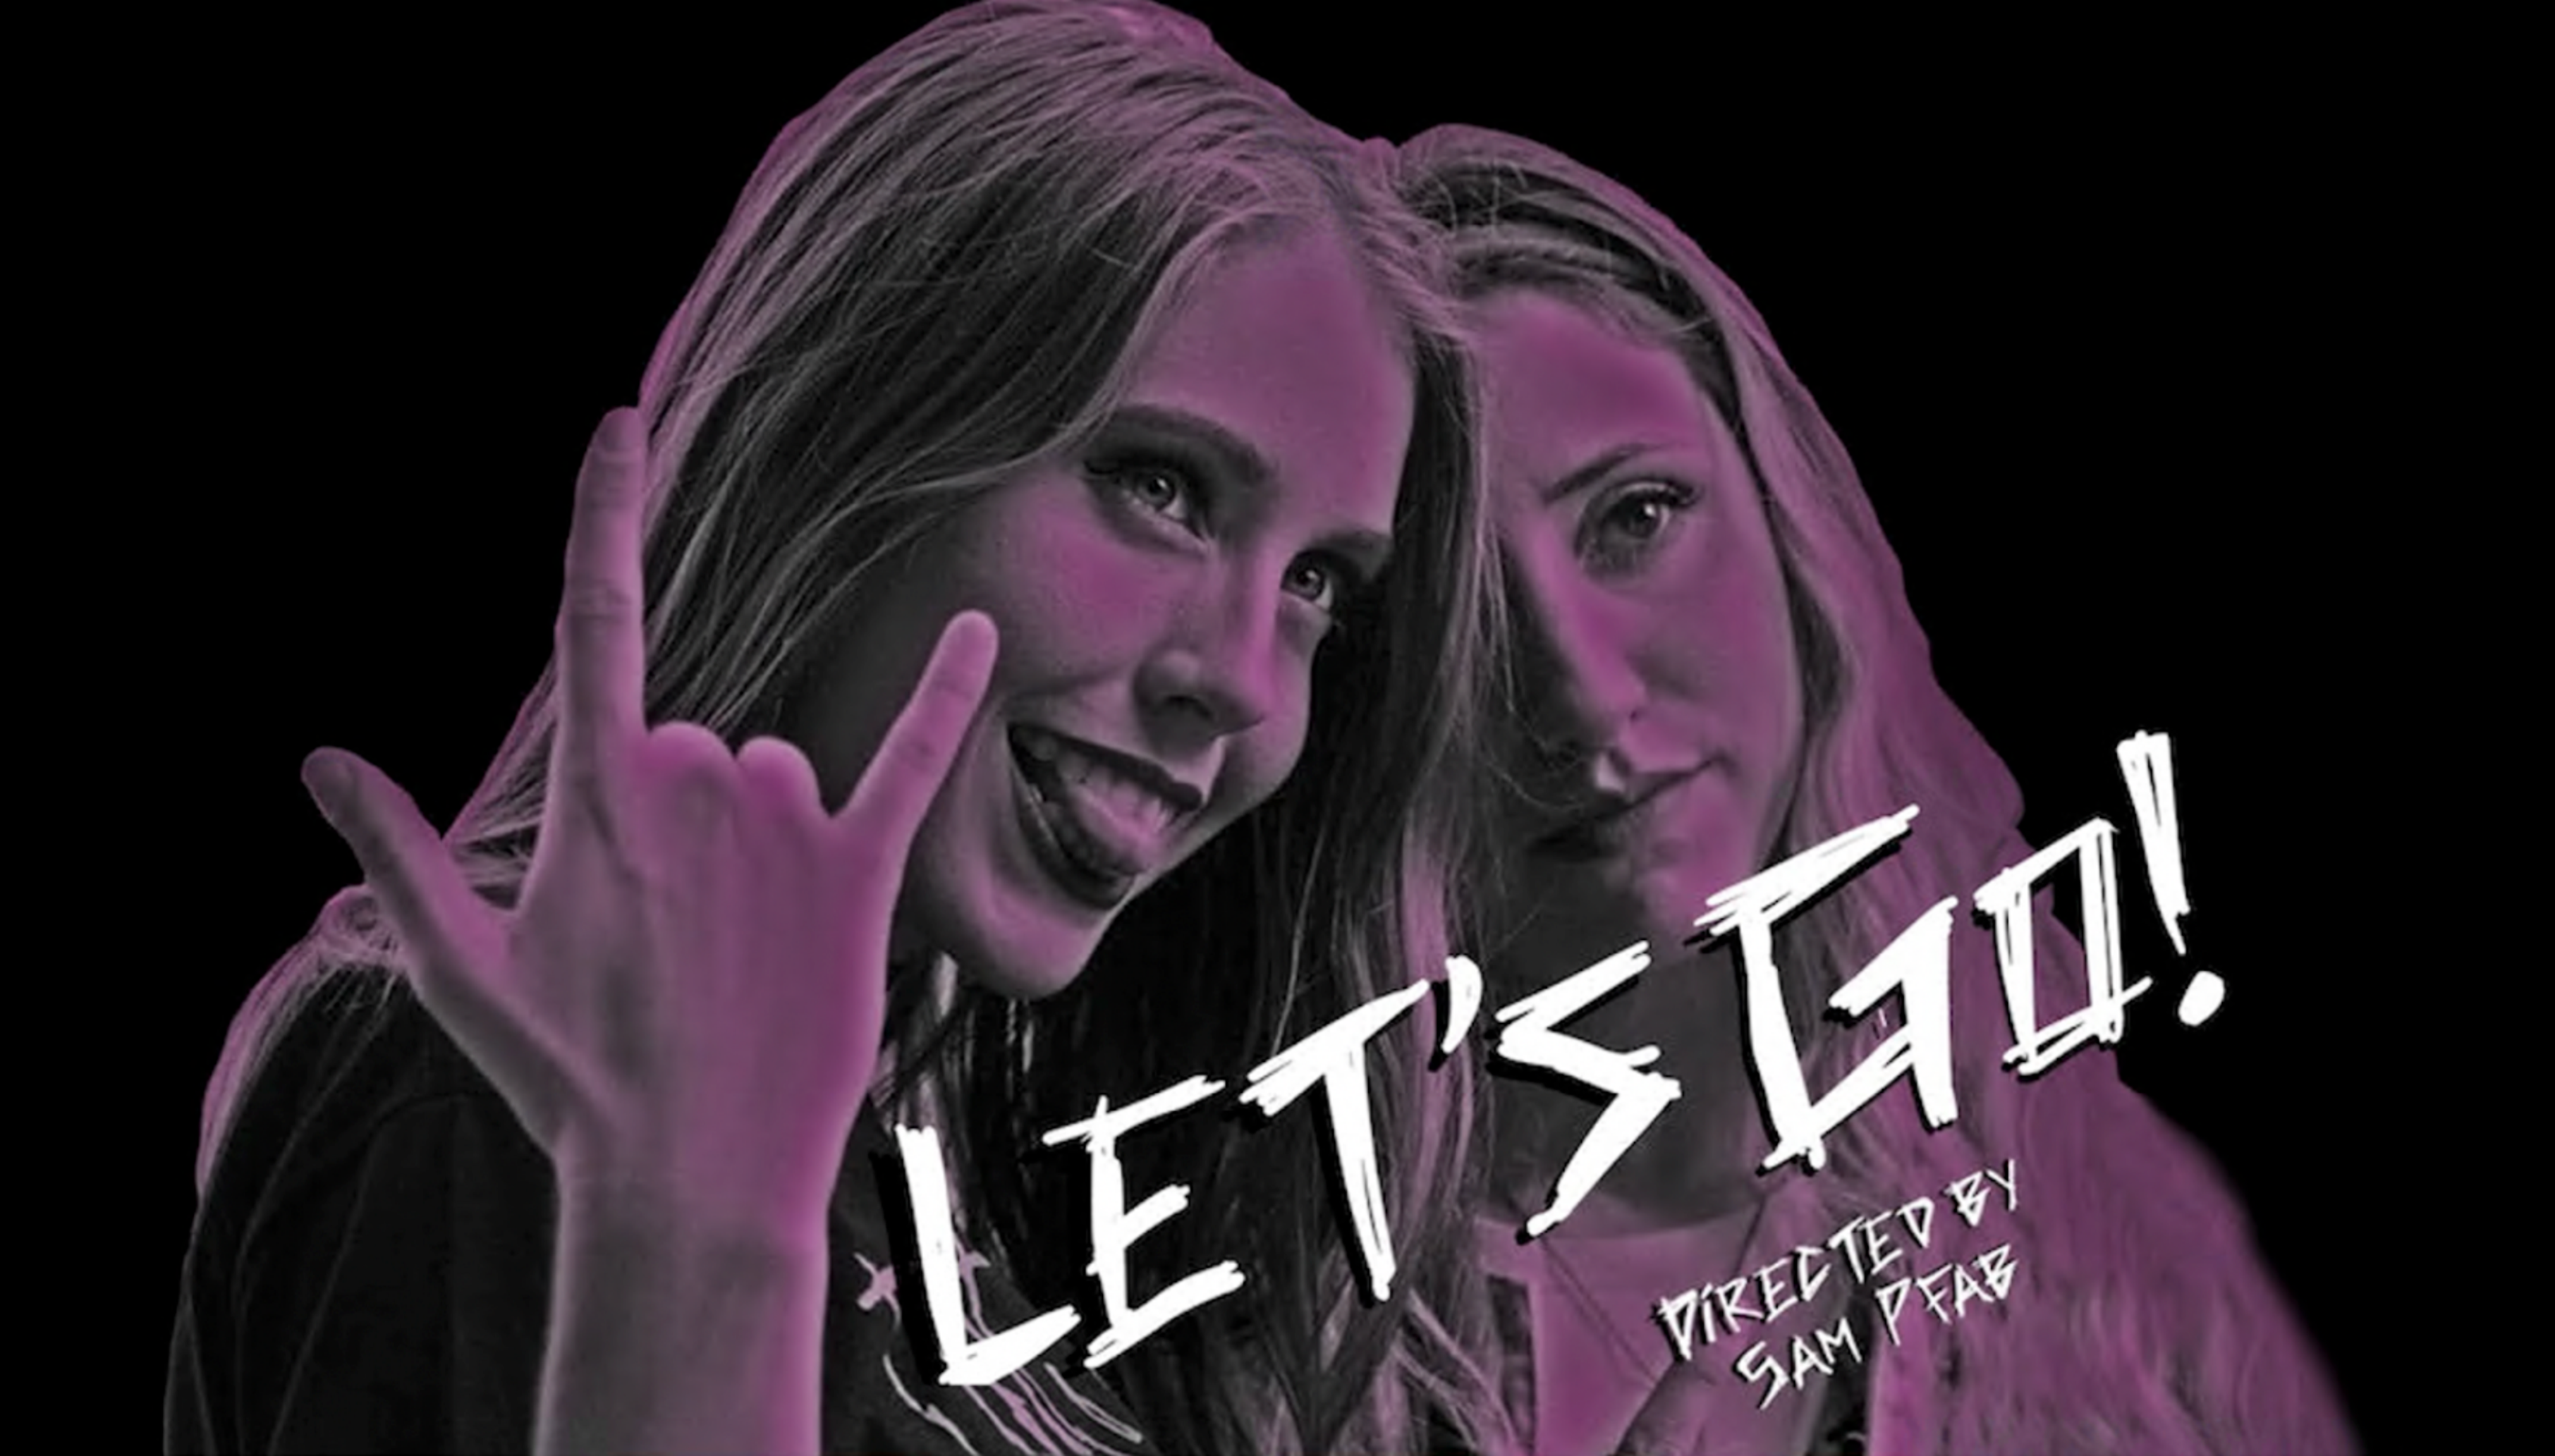
\includegraphics[width=8.5cm]{Figures/record_store_protest-2.pdf}
\vspace{-1.3em}
\caption{An example pair of image and human caption text from our crowdfunding dataset. The caption generated by the BLIP model and the actual human-generated caption of the image is below. 
\textbf{BLIP caption:} "Two women smiling with a hand gesture of rock and roll." 
\textbf{Actual human caption:} "Smash the glass ceiling. Destroy the patriarchy. Save the record store."}
\vspace{-1em}
\label{fig:image-womens-movement-patriachy}
\end{figure} 

Table \ref{tab:generated-caption-two-women} provides the generated explanations using SOTA multimodal models including BLIP2, and LLava. 
%Overall, 
While LLava \cite{liu2023visual} did generate explanations of the input pair with a  contextually informed meaning, it suffers from hallucinations, such as “The image features two women standing next to each other, \emph{both holding their cell phones in their hands. They seem to be taking selfies}”. In the given image, there are no cell phones nor are they taking selfies.
%is no sign of women holding their cell phones.
%, while the model claims otherwise. 
For comparison, we queried ConceptNet {\cite{speer2018conceptnet}} to extract the most relevant concepts, and simply appended these to the pair of text and image as input to these models. As expected, the generated output does mitigate hallucinations (see Table \ref{tab:generated-captions} in Appendix). This %point is 
shows that multimodal analysis guided by external knowledge %improves performance by making 
makes more reliable inferences by forming cross-modal contextual connections. 

%Researchers have studied the hallucination problem in several use cases including text summarization \cite{huang2021factual} and dialogue generation \cite{shuster2021retrieval}, showing how retrieval-augmented multimodal models can generate enhanced and grounded representations with external knowledge. 

%One problem with existing methods is a lack of congruence between the interpretation of the image and the associated text. 
%Our emphasis on multimodal congruence introduces a measurement problem. 
We introduce here the notion of \emph{multimodal congruence.} We measure multimodal congruence 
%learned by multimodal models 
%through measuring the 
using the semantic distance between the separate image and caption (text) representations, 
as this distance is 
expected to be shorter in a congruent multimodal representation \cite{mandera2017explaining,frank2017word,beck2011congruence,maki2004semantic}. We can then demonstrate how external knowledge can enhance and contextualize the representations to close the semantic gap between the modalities. In doing so, we can better predict the success of marketing campaigns.  
% TK: Interesting discussion - if you can later present how to generate an embedding of the semantics of image and caption and formally measure their distance and then motivate how to bridge it with what consequence, it will be neat!

%Our approach incorporates external knowledge in a multimodal learning framework. 
In this study, we answer the following two research questions: \\
\textbf{RQ1:} Can we 
%explore and 
improve the contextual congruence of the representations of multimodal content by incorporating external knowledge while learning to unveil subtle cross-modal semantic relationships? \\
\textbf{RQ2:} Do more contextually congruent representations help the model obtain more consistent and reliable predictive performance for the success of multimodal marketing campaigns? %effectiveness? 

Our technical approach incorporates  an external commonsense Knowledge Graph (KG) (e.g., ConceptNet) 
%incorporated 
to learn knowledge-infused multimodal representations of the data. We first take pairs of images and text from our dataset and generate embeddings using text and image encoders (i.e., via LLMs, LVMs). To query the KG, %ConceptNet, 
we generate captions for images using BLIP \cite{li2022blip}. Then, we retrieve the most similar concepts from ConceptNet based on semantic search. We train knowledge graph embedding (KGE) models to generate representations of the resulting concepts. Initially, we learn multimodal data representations using bidirectional transformers. These representations are then fused with the KGEs through a linear and a multi-head cross-attention layer. 

The novelty of our work lies in modeling a social and behavioral problem, such as effective marketing, utilizing neural and symbolic models \cite{sap2022neural}. In so doing, we particularly addressed the problem of learning a contextually enhanced neural representation of multimodal content with external commonsense KG (i.e., symbolic) \cite{yu2022probabilistic,kursuncu2020kil}. This helps the model to better capture the holistic meaning across modalities enhancing model performance in predicting the success of multimodal marketing campaigns.
% %Our experiments involving 
% Utilizing multiple LLMs and LVMs coupled with KGEs, we demonstrate the 
% %difference in 
% performance advantage for predicting the success of multimodal marketing campaigns.  
%We observe that the 
%Representations enhanced with explicit contextual information help models form semantic connections between modalities. 
Knowledge-infused multimodal models outperform other models without knowledge. Error analysis (see Section Results \& Discussion) reveals how external knowledge improves the capture of intended holistic multi-modal meaning. 
%Thus, we simultaneously 
We demonstrate the contribution of knowledge to machine learning algorithms 
%and to enable 
for computational analysis of marketing campaigns, which provide an ecologically valid measure of success.
%To clarify the contribution of knowledge, we provide a discussion on error analysis in our experiments as to how external knowledge improves the capturing of the intended meaning.
%This contextualization proves to be impactful in a downstream task in marketing. 
%While t
%The findings indicate the critical contribution of external knowledge from a KG to the machine understanding of multimodal content.
%, there is much to explore in incorporating knowledge for contextualizing multimodal representations.

\begin{table*}[hbt!]
\vspace{-0.2em}
  \centerline{
    \begin{tabular}{p{0.8cm}p{1.3cm}p{14.2cm}}
    \toprule[2pt]
   \textbf{\centering Model} & \textbf{\centering Knowledge} & \textbf{Text Caption} \\
    \toprule[1pt]
    BLIP2 & \centering No & the cover of let's go with two girls posing in front of a purple background going for a protest. \\
    \toprule[1pt]
    BLIP2 & \centering Yes & The cover of a movie "let's go" which talks about patriachy in the record store. \\ 
    \toprule[1pt]
    Llava & \centering No & The image features two women standing next to each other, both holding their cell phones in their hands. They seem to be taking selfies or sharing a moment together. One of the women is making a funny face, adding a playful vibe to the picture. The other woman is simply enjoying the moment and being part of the fun. \\ 
    \toprule[1pt]
    Llava & \centering Yes & The image features two beautiful and majestic black women standing together, united in their quest to smash the glass ceiling and destroy the patriarchy. They are surrounded by record albums, highlighting their shared passion for music and the record store. Their powerful presence and determination to save the record store from any threat make for a compelling scene that showcases their strength and resilience in the face of oppressive societal norms. \\
    \bottomrule[2pt]
    \end{tabular}%
  }
\vspace{-0.5em}
\caption{For the image and text pair (see Figure \ref{fig:image-womens-movement-patriachy}), the captions generated by the models BLIP2 and Llava, when the model was prompted with the Image and Text with and without external Knowledge. The knowledge is extracted from ConceptNet as explained in section \ref{sec:explicit-knowledge} and appended to the prompt input to these models. 
%While t
\emph{The captions with generated knowledge show less hallucination.}
% and more grounding, we leave further investigation of those to the reader as they are not the focus of this study. 
For more examples, see Table \ref{tab:generated-captions} in the Appendix.}
\label{tab:generated-caption-two-women}
% \vspace{-0.2em}
\end{table*}

\vspace{-0.5em} 
\section{Background \& Related Work}
\label{sec:related}
\input{Relatedwork}


\vspace{-1mm}
\section{Preliminaries}
\label{sec:prelim}
\input{Preliminaries}


\vspace{-0.5em} 
\section{Exploratory Analysis}
\label{sec:exploratory}
\input{Exploratoryanalysis}


\vspace{-0.5em} 
\section{Methods}
\label{sec:methodology}
\input{Methodology}


\vspace{-0.5em} 
\section{Results \& Discussion}
\label{sec:results-discuss}
\input{ResultsDiscussion}

% \section{Error Analysis}
% \label{sec:error-analysis}
% \input{aaai2024/11-Erroranalysis}


\vspace{-0.8em} 
\section{Conclusion}
\label{sec:conclusion}
\input{Conclusion}

% \clearpage
% \newpage

% Entries for the entire Anthology, followed by custom entries
\bibliography{references}

\clearpage

% \section{Paper Checklist}
% \label{sec:paper-checklist}
% \input{aaai2024/8-Checklist}
% \appendix

\clearpage

\section{Appendix}
\label{sec:otherappendix}
\subsection{Implicit and Explicit Context}
\label{sec:implicit-explicit-context}
Implicit context refers to the latent relationships and dependencies inferred by capturing the surrounding information environment through mechanisms, such as self-attention for transformers, gating for RNNs, and co-occurrence for Word2Vec. More specifically, the self-attention mechanism 
%allows the model to attend 
guides the model by assigning different weights to more relevant parts of the input sequence to capture dependencies between elements.
Explicit context refers to the information that is clearly stated in the content (e.g., text, image) without requiring additional interpretation or inference to understand. It is provided 
%explicitly provided 
alongside the input sequence to enhance its representation and understanding. Knowledge graphs and ontologies can be used to provide this contextual information as external knowledge. We utilize ConceptNet in this study, which provides external knowledge as a structured representation of real-world concepts and their relationships.

\subsection{Knowledge Embedding Models}
\label{sec:knowledge-embedding-models}

Knowledge graph embeddings, also known as knowledge graph representation learning, are techniques used to represent entities and relationships as dense, low-dimensional vectors. These embeddings capture the semantic relationships and similarities between entities and allow for efficient computation and reasoning in knowledge graph-based tasks. In our study we refer to the knowledge graph as $K_g$. Each triple in $K_g$ is represented as $(h,r,t)$ where the entities relation, head and tail are represented as  $h$, $r$ and $t$ respectively.

\textbf{TransE} \cite{bordes2013translating} is a translational energy-based model that represents entities and relations as vectors of the same Euclidean space $R^d$. For a given triple, score function is defined as $f_r(h,t) = -||h+r-t||_{l_1,l_2}$.
% In terms of vector computation it could be represented as or $ h + r \approx t$. 
% TransE performs linear transformation using the following scoring function:

% \begin{equation}
% f = -\lVert h+r-t \rVert_{\frac{1}{2}}
% \end{equation}
\textbf{RotateE} \cite{sun2019rotate} is a translational based model that represents entities and relations in complex vector space $C^d$ and defines each relation as an element-wise rotation from the head entity to the tail entity. The score function is formulated as $f_r(h,t) = - ||h\odot r - t||$, where $\odot$ is the Hadamard (or element-wise) product. 

\textbf{DistMult} \cite{yang2014embedding} DistMult is a semantic-matching model, where the score of a triple can be computed as the bilinear product which is represented as $f_r(h,t) = h\times r \times t$ where $e_h,e_t \in R^d$ and $r \in R^{d \times d}$. Here, restricting $R$ to a diagonal matrix, the score is computed as $f_r(h,t) = h\times diag(r) \times t$.
% In DistMult, every relation $r$ is represented by a diagonal matrix $M_{r}  \in {R}^{{d} \times {d}}$ and a triple is scored as $f(h,r,t) = {e_h}^TM_rE_t$ where $e_h,e_t \in R^d$.
% and a triple is scored as:

% \begin{equation}
% f(h,r,t)= e^{T}_{h} M_{r} e_{t}
% \end{equation}

\subsection{Example data points with captions}
The following examples are from our dataset. Similar to the example in Section \ref{sec:intro} and Table \ref{tab:generated-caption-two-women}, we generated captions with and without knowledge for Figures \ref{fig:muslim-cap} and \ref{fig:ruler} and provided in Table \ref{tab:generated-captions}.  

\begin{figure}[hbt!]
  \centering
  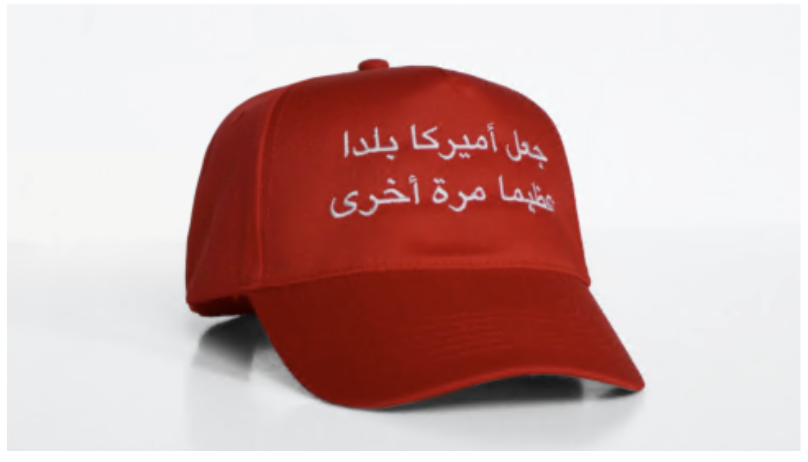
\includegraphics[width=8.5cm]{Figures/muslim_cap.png}
\vspace{-1em}
\caption{\textbf{Actual caption:} "Let's remind everyone that Muslim Americans are a part of our country and that they, too, make America great."}
% \vspace{-1.5em}
\label{fig:muslim-cap}
\end{figure} 

\begin{figure}[hbt!]
  \centering
  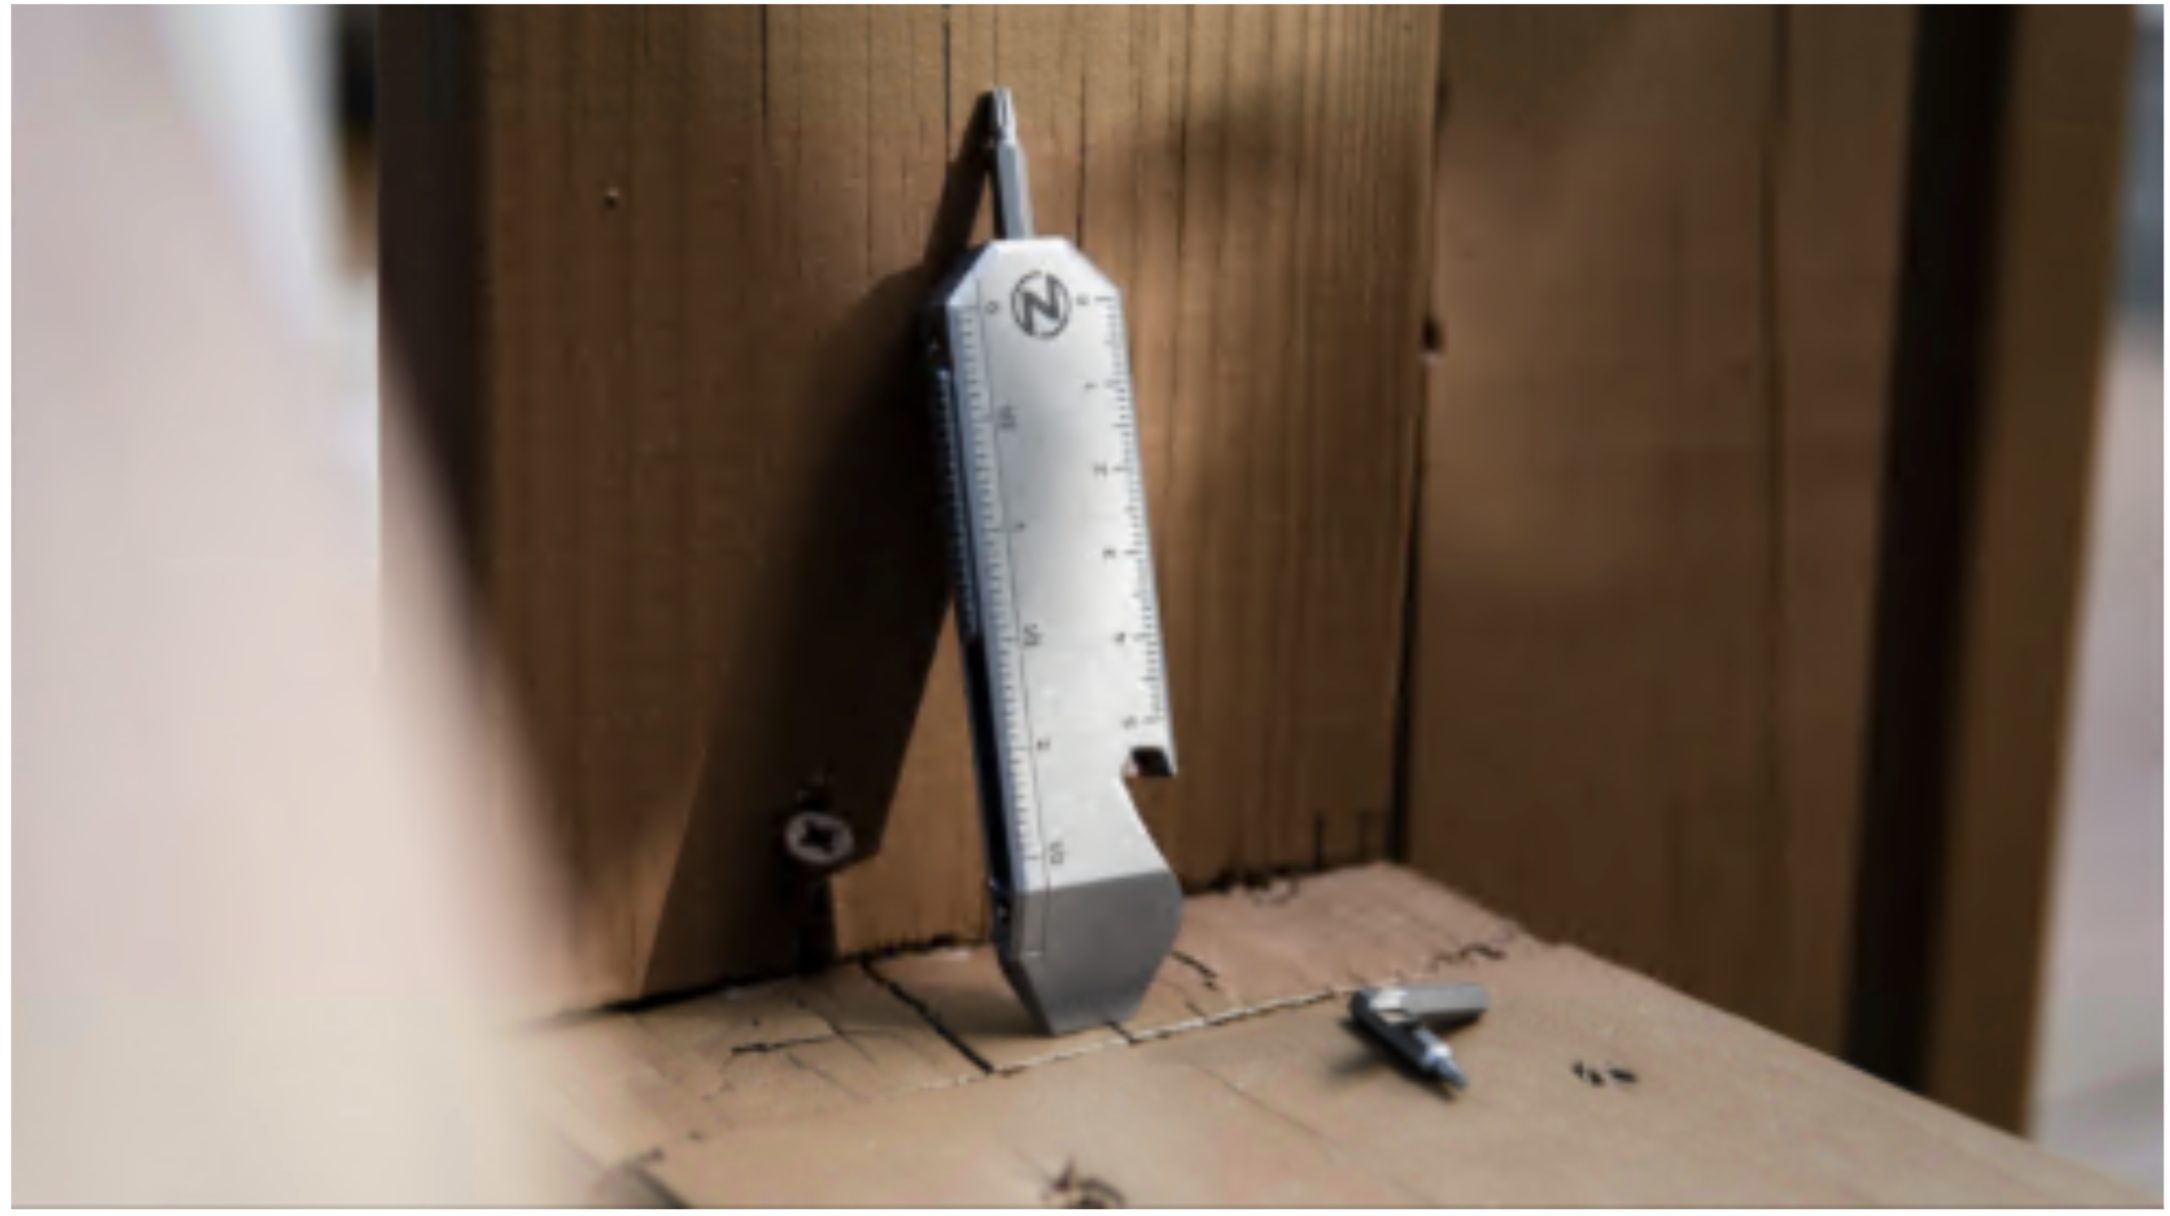
\includegraphics[width=8.5cm]{Figures/ruler.png}
% \vspace{-1em}
\caption{ \textbf{Actual caption:} " A TSA-compliant multi-tool with an innovative internal bit storage compartment"}
\vspace{-1.5em}
\label{fig:ruler}
\end{figure} 

\begin{table*}[!htbp]
  % \setlength\extrarowheight{-2pt}
  \centerline{%
    \begin{tabular}{p{1cm}p{2cm}p{10cm}p{1cm}}
    \toprule[3pt]
   \textbf{Model} & \textbf{Knowledge} & \textbf{Caption} & \textbf{Figure Label} \\
    \toprule[1pt]
    BLIP2 & No& a red baseball cap with arabic writing on it & \ref{fig:muslim-cap} \\
    \toprule[1pt]
    BLIP2 & Yes & muslim Americans are a part of our country and that they, too, make America great
    & \ref{fig:muslim-cap} \\ 
    \toprule[1pt]
    Llava & No & The image features a red cap with white lettering, likely a "Make America Great Again" hat, positioned on a white surface. The hat has Arabic writing on it, suggesting it is meant to convey a message of inclusivity and support for Muslim Americans. The message on the cap reads, "Muslim Americans also make America great." This serves as a reminder that Muslim Americans contribute significantly to the country and are essential in making America great, just like individuals from various backgrounds. & \ref{fig:muslim-cap} \\ 
    \toprule[1pt]
    Llava & Yes & The image features a red cap with white lettering, likely a "Make America Great Again" hat, placed on a white surface. The hat displays Arabic writing, which says, "Muslim Americans also make America great." This message emphasizes the importance of recognizing and appreciating the contributions of Muslim Americans to the nation, reminding people that they, too, play a vital role in making America great. The concept of Americanization refers to the process of adapting to American culture, values, and traditions, and this hat promotes the idea of Muslim Americans actively participating in and enriching the American society. & \ref{fig:muslim-cap} \\ 
    \toprule[3pt]
    BLIP2 & No &  a ruler is sitting on top of a piece of wood
    & \ref{fig:ruler} \\ 
    \toprule[1pt]
    BLIP2 & Yes &  a ruler is sitting on top of a piece of wood
    & \ref{fig:ruler} \\ 
    \toprule[1pt]
    Llava & No &  The image features a silver ruler with an internal bit storage compartment, placed against a brown wooden background. The ruler appears to be a TSA-compliant multi-tool, designed for both measuring and carrying small tools securely while in transit. The ruler's unique storage feature allows it to hold bits or other small objects, making it a practical and convenient tool for various purposes.
    & \ref{fig:ruler} \\ 
    \toprule[1pt]
    Llava & Yes & The image features a silver ruler with an internal bit storage compartment, designed for carrying and organizing small tools or bits securely. \textbf{This TSA-compliant multi-tool is particularly useful for transporting and organizing military equipment or cargo, as it can easily fit into the compartments of aircraft. The innovative internal storage compartment allows for efficient use of space, making it a very handy tool to carry and transport in unmanned transportation devices or the cargo hold of aircraft}
    & \ref{fig:ruler} \\ 
    \bottomrule[3pt]
    \end{tabular}%
  }
\caption{For the image and text pairs (see Figures \ref{fig:muslim-cap} and \ref{fig:ruler}), the captions generated by the models BLIP2 and Llava, when the models were prompted with the Image and Text with and without external Knowledge. The knowledge is extracted from ConceptNet as explained in section \ref{sec:explicit-knowledge} and appended to the prompt input to these models. While the generated captions with knowledge show less hallucinations and more grounding, we leave further investigation of those to the reader as they are not the focus of this study.}
\label{tab:generated-captions}
\end{table*}


\subsection{Extended Exploratory Analysis}[hbt!]
Similar to what we did in the exploratory analysis described in Section \ref{sec:exploratory}, we created clusters for text and image modalities, but in different sizes this time, to show that our observations did not change as shown in Figure \ref{fig:context_congruence_across_data_size}. The clusters get denser and the centroids get closer between them. 


\begin{figure*}
  \centering
  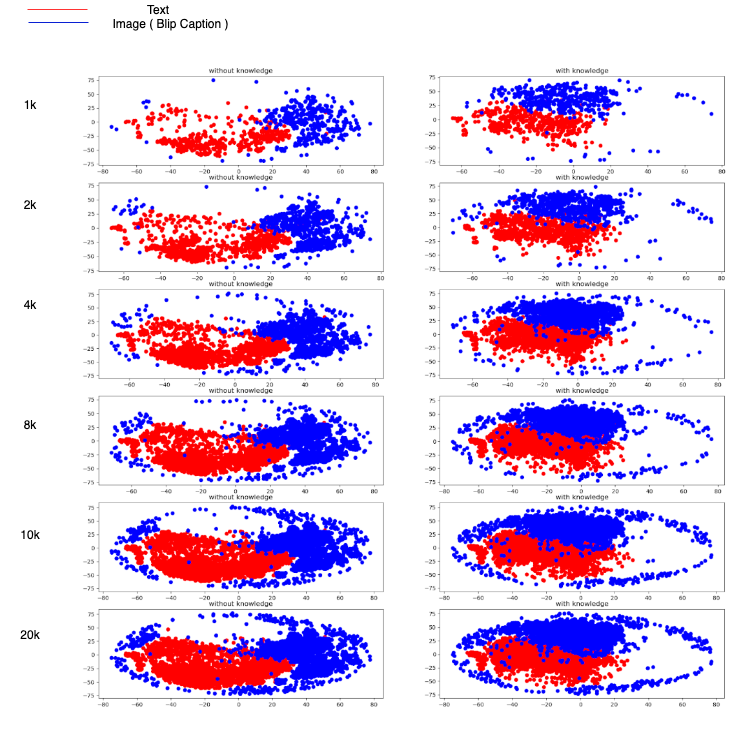
\includegraphics[width=18cm]{Figures/context_congruence_across_data_size.png}
% \vspace{-1em}
\caption{Cluster of the Embeddings of the BLIP Captions and the Marketing Caption Embeddings across varying data sizes. The gap between the image and text clusters reduces in the right plot with the addition of knowledge and can be seen across varying data sizes}
\vspace{-1.5em}
\label{fig:context_congruence_across_data_size}
\end{figure*} 


\subsection{Error Analysis Examples}
As we provided two examples for discussing different outcomes from our experiments including positive and negative, here we provide more examples for the reader to investigate further. The examples include Figures and their explanations
For Figure \ref{fig:error-analysis-woofer-error-analysis}, 
% \textbf{Explanation:} 
The campaign image promotes their 'subwoofer', 'dsp' solution by showing  ‘crowd\_concert’  of fans, their hands raised high in the air. It helps to convey the message  'many\_people\_to\_attend\_concert’.
For Figure \ref{fig:music-album-error-analysis}, 
% \textbf{Explanation:} 
The campaign ad is for a band which wants to promote its music by selling merchandise and by making  its digital copies and their merchandise available for purchase on their website. The band featured in the campaign ad wants to connect with their audience by providing specialized merchandise and releasing their music in digital formats. The noisy entities from the conceptnet ['bridge\_distance\_between\_people', 'bridge', 'bridges', 'bridgeness', 'holding\_up\_bridge']  fail to capture the important events in the pair of image and text.
For Figure \ref{fig:error-analysis-poetry-graffiti}, 
% \textbf{Explanation:} 
The campaign aims to showcase the intersection of 'performance\_poetry' by 'filmmaking'  by capturing these artistic expressions in unconventional locations such as  'graffiti' on  'front\_wall'.The campaign seeks to celebrate both the poet performers and the 'graffitists'.
For Figure \ref{fig:error-analysis-sucess-poet} 
% \textbf{Explanation:} 
Explanation : The campaign image showcases ‘poetry\_book’, ‘books\_of\_poems’, positioned over the ‘wooden\_table’ or the ‘book\_table’.
For Figure \ref{fig:error-analysis-failure-custom-windows}, 
% \textbf{Explanation:} 
The campaign ad is of a company named  “CUSTOMATIC”  which designs custom windows. lot of noisy concepts retrieved such as ‘word\_picture’ which get infused, may confuse the model.


% \vspace{-1.5em}
% \label{fig:custom-windows-error-analysis}
% \end{figure} 

\begin{figure}[hbt!]
  \centering
  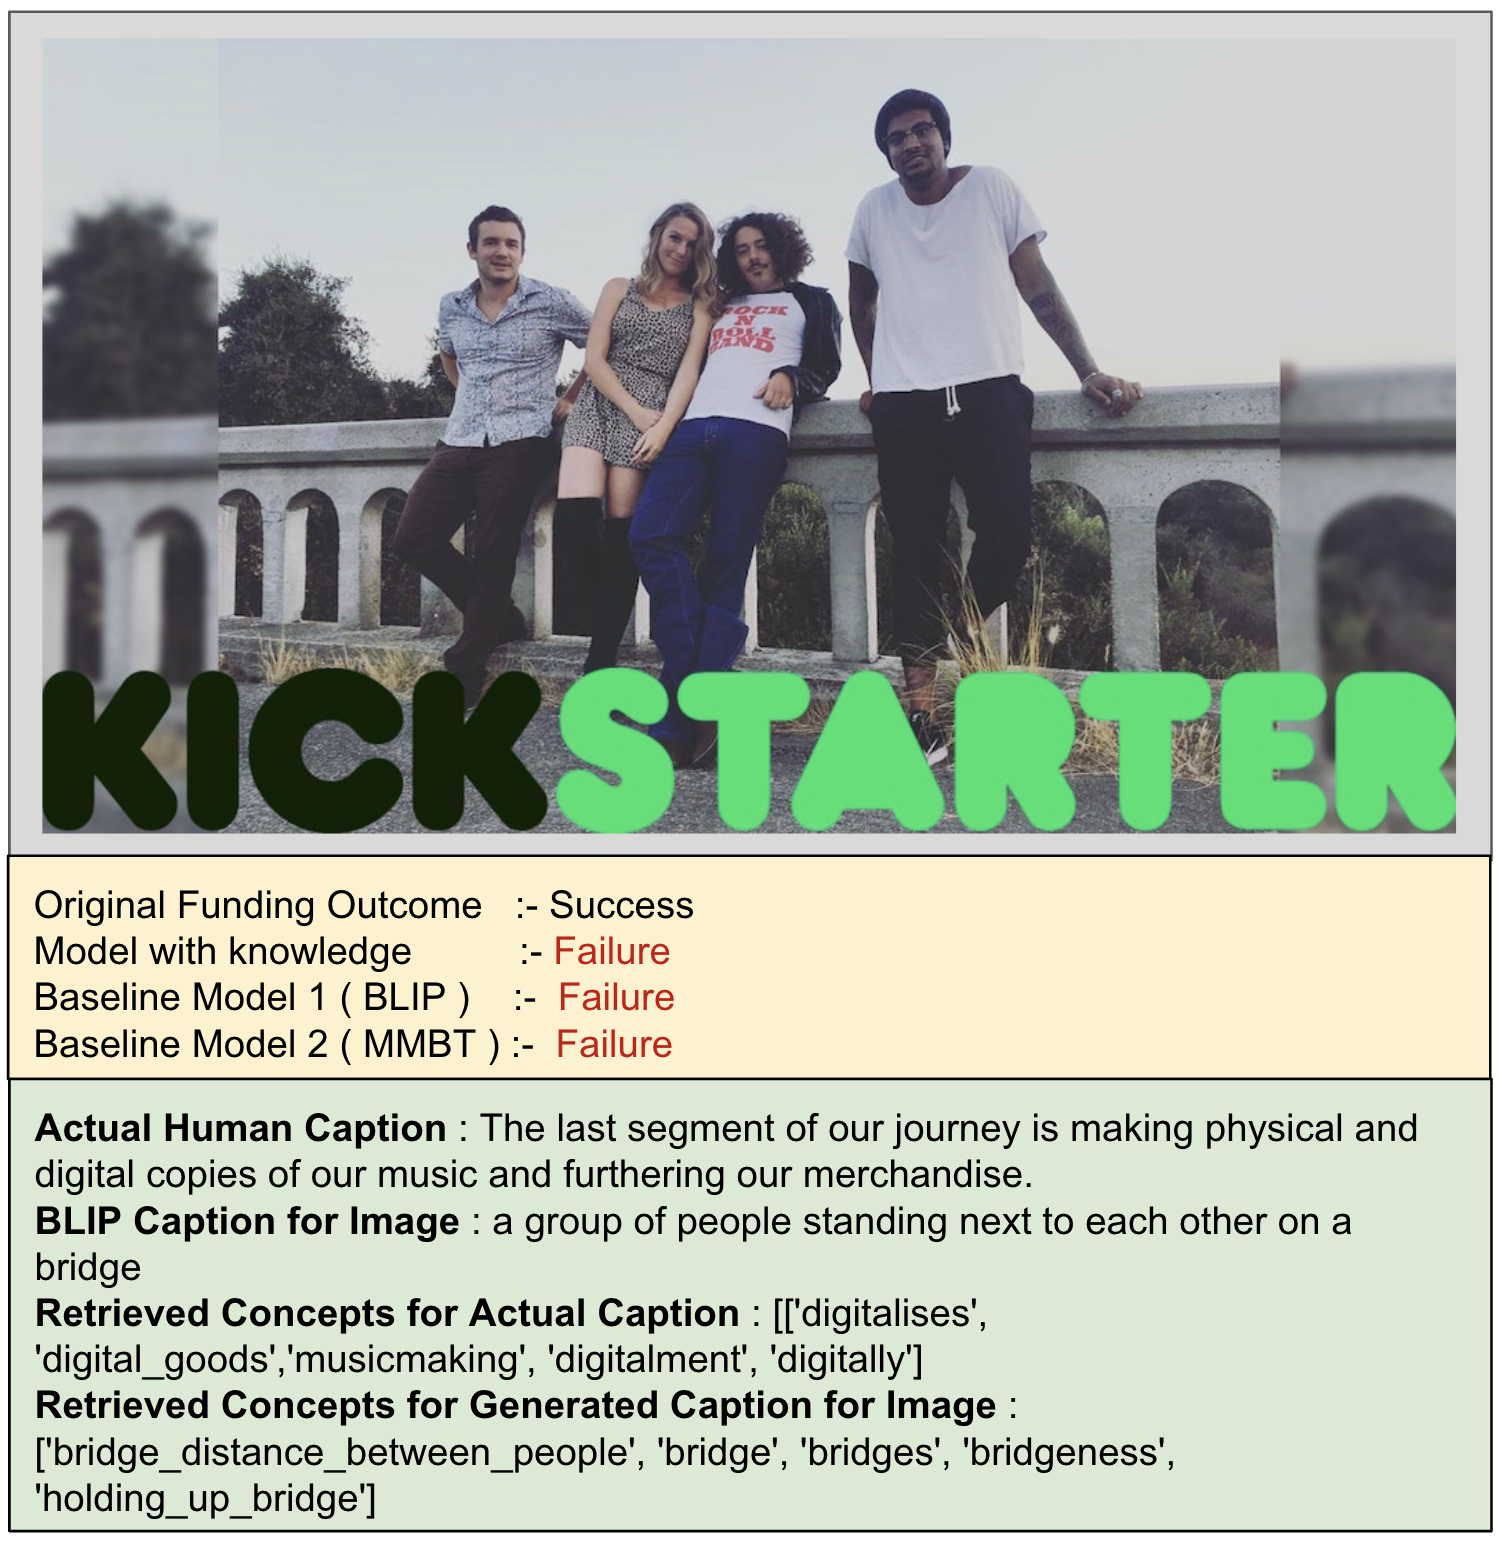
\includegraphics[width=8.5cm]{Figures/erroranalysis/error-analysis-music-band.png}
% \vspace{-1em}
\caption{In the yellow box, the prediction of the model with knowledge, blip model and MMBT, In the green box, actual caption, blip caption, retrieved concepts for each modality.}
\vspace{-1.5em}
\label{fig:music-album-error-analysis}
\end{figure} 

\begin{figure}[hbt!]
  \centering
  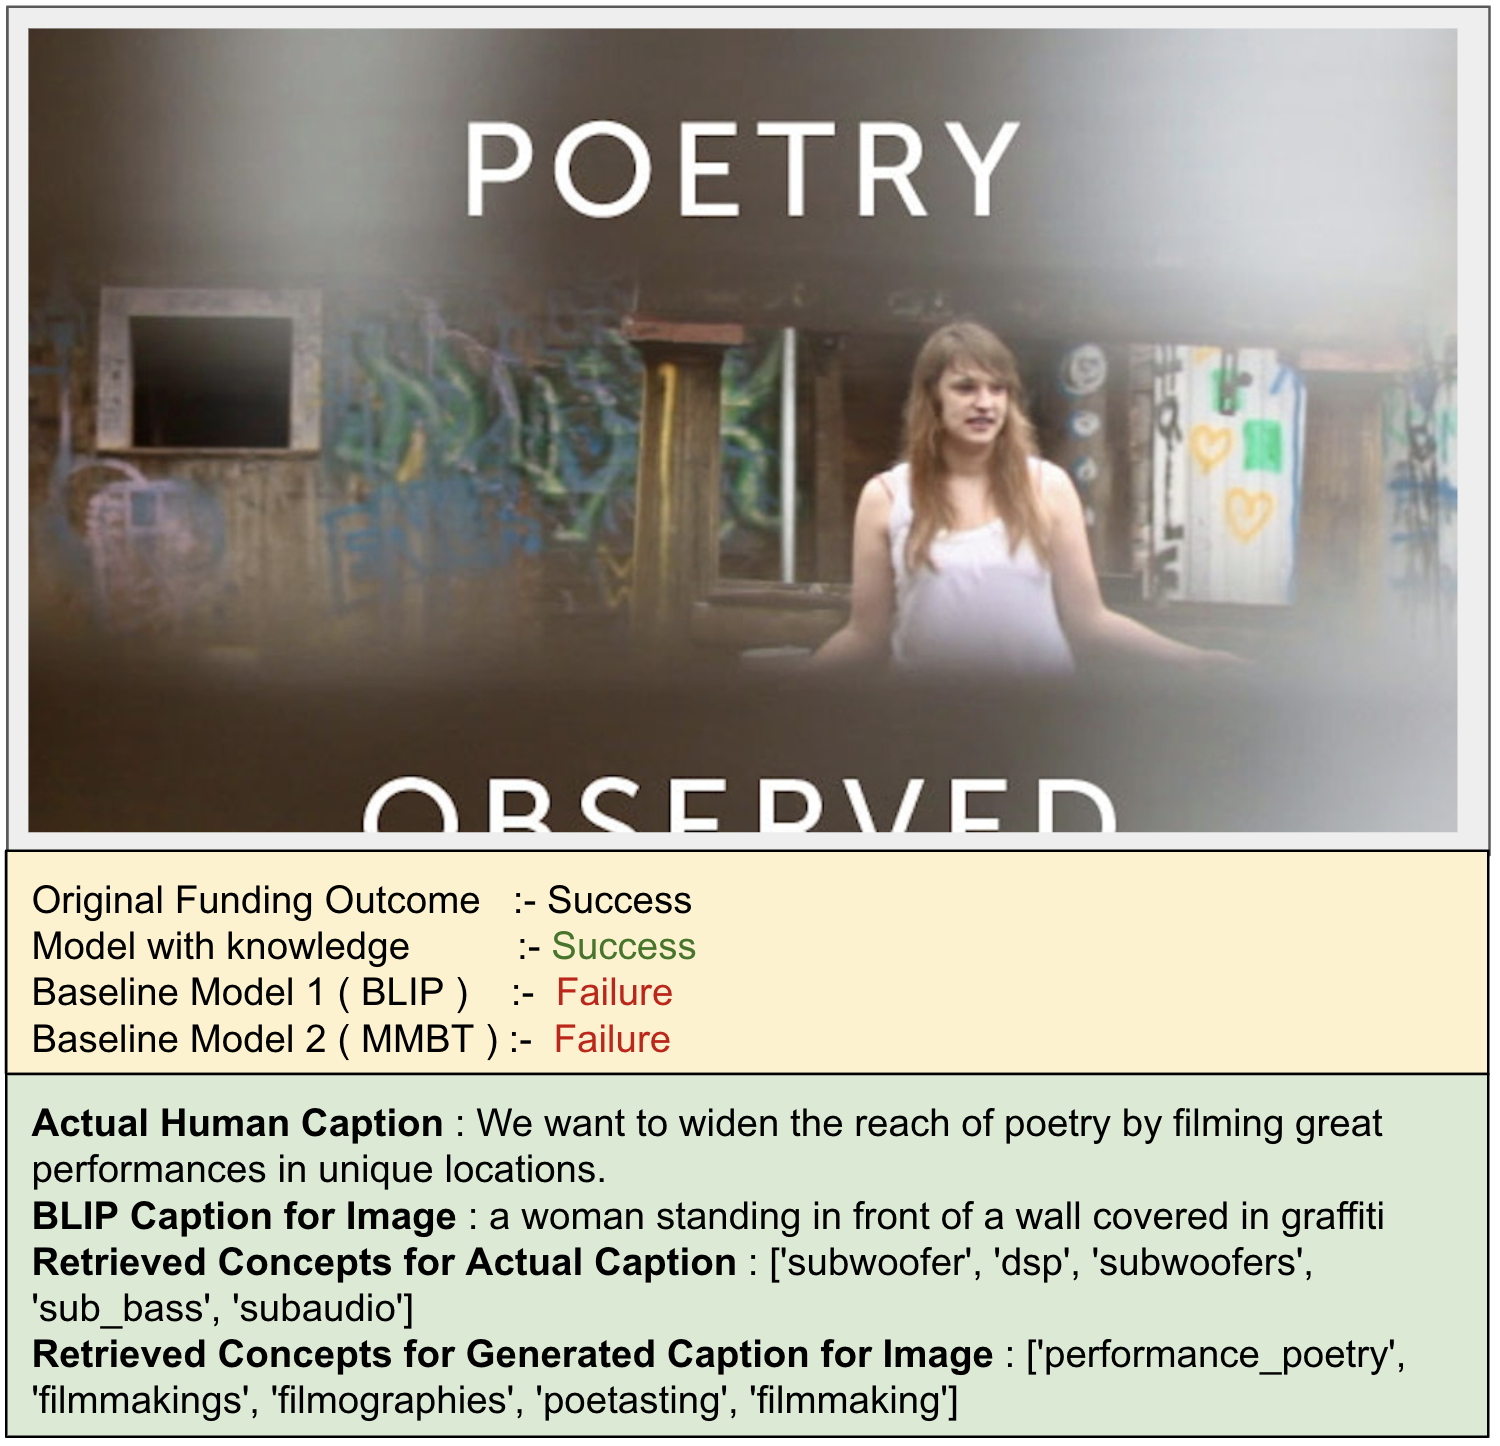
\includegraphics[width=8.5cm]{Figures/erroranalysis/error-analysis-sucess-poet-graffiti.png}
% \vspace{-1em}
\caption{In the yellow box, the prediction of the model with knowledge, blip model and MMBT, In the green box, actual caption, blip caption, retrieved concepts for each modality.\\ 
}
\vspace{-1.5em}
\label{fig:error-analysis-poetry-graffiti}
\end{figure} 


\begin{figure}[hbt!]
  \centering
  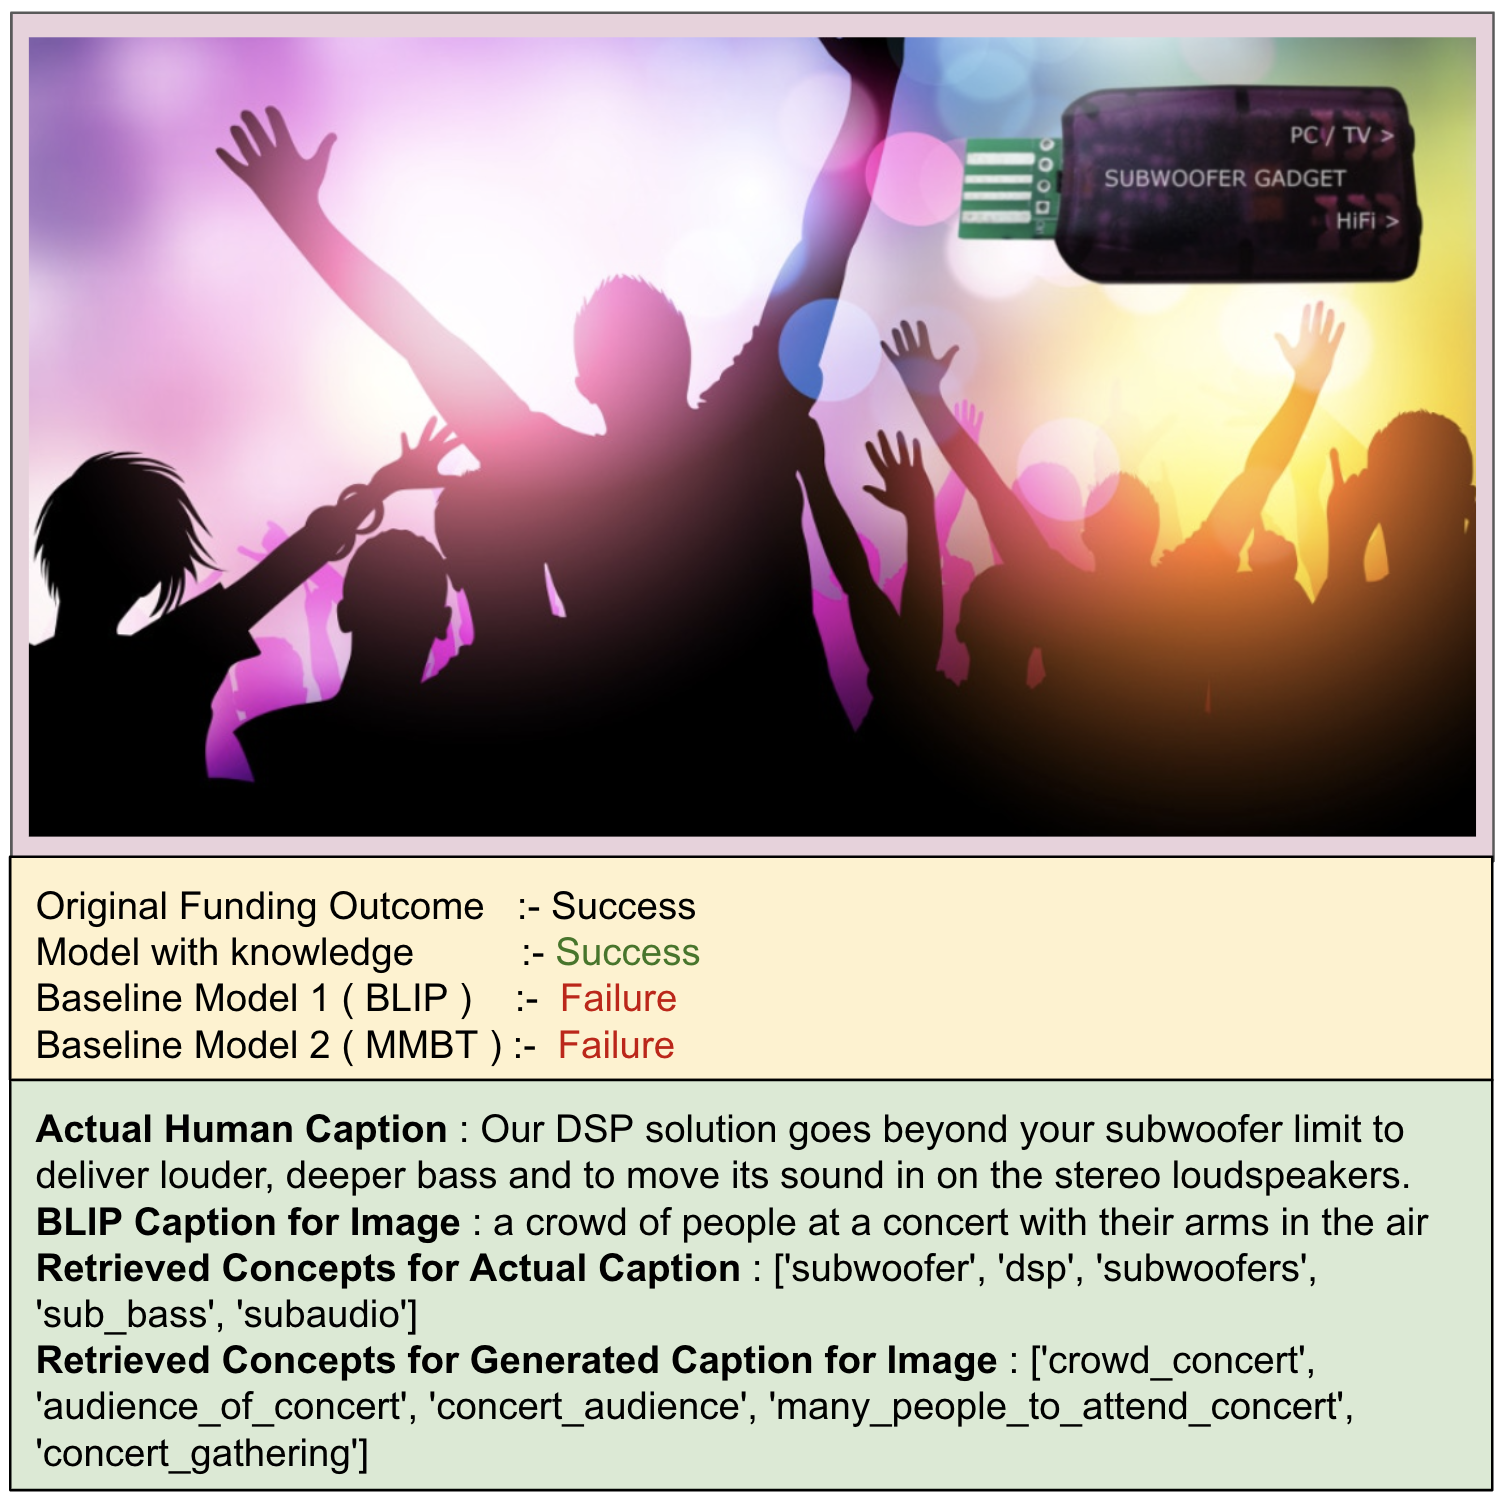
\includegraphics[width=8.5cm]{Figures/erroranalysis/error-analysis-sucess-woofer.png}
% \vspace{-1em}
\caption{In the yellow box, the prediction of the model with knowledge, blip model and MMBT, In the green box, actual caption, blip caption, retrieved concepts for each modality are shown.\\
% \textbf{Explanation:} The campaign image promotes their 'subwoofer', 'dsp' solution by showing  ‘crowd\_concert’  of fans, their hands raised high in the air. It helps to convey the message  'many\_people\_to\_attend\_concert’.
}
\vspace{-1.5em}
\label{fig:error-analysis-woofer-error-analysis}
\end{figure} 

\begin{figure}[hbt!]
  \centering
  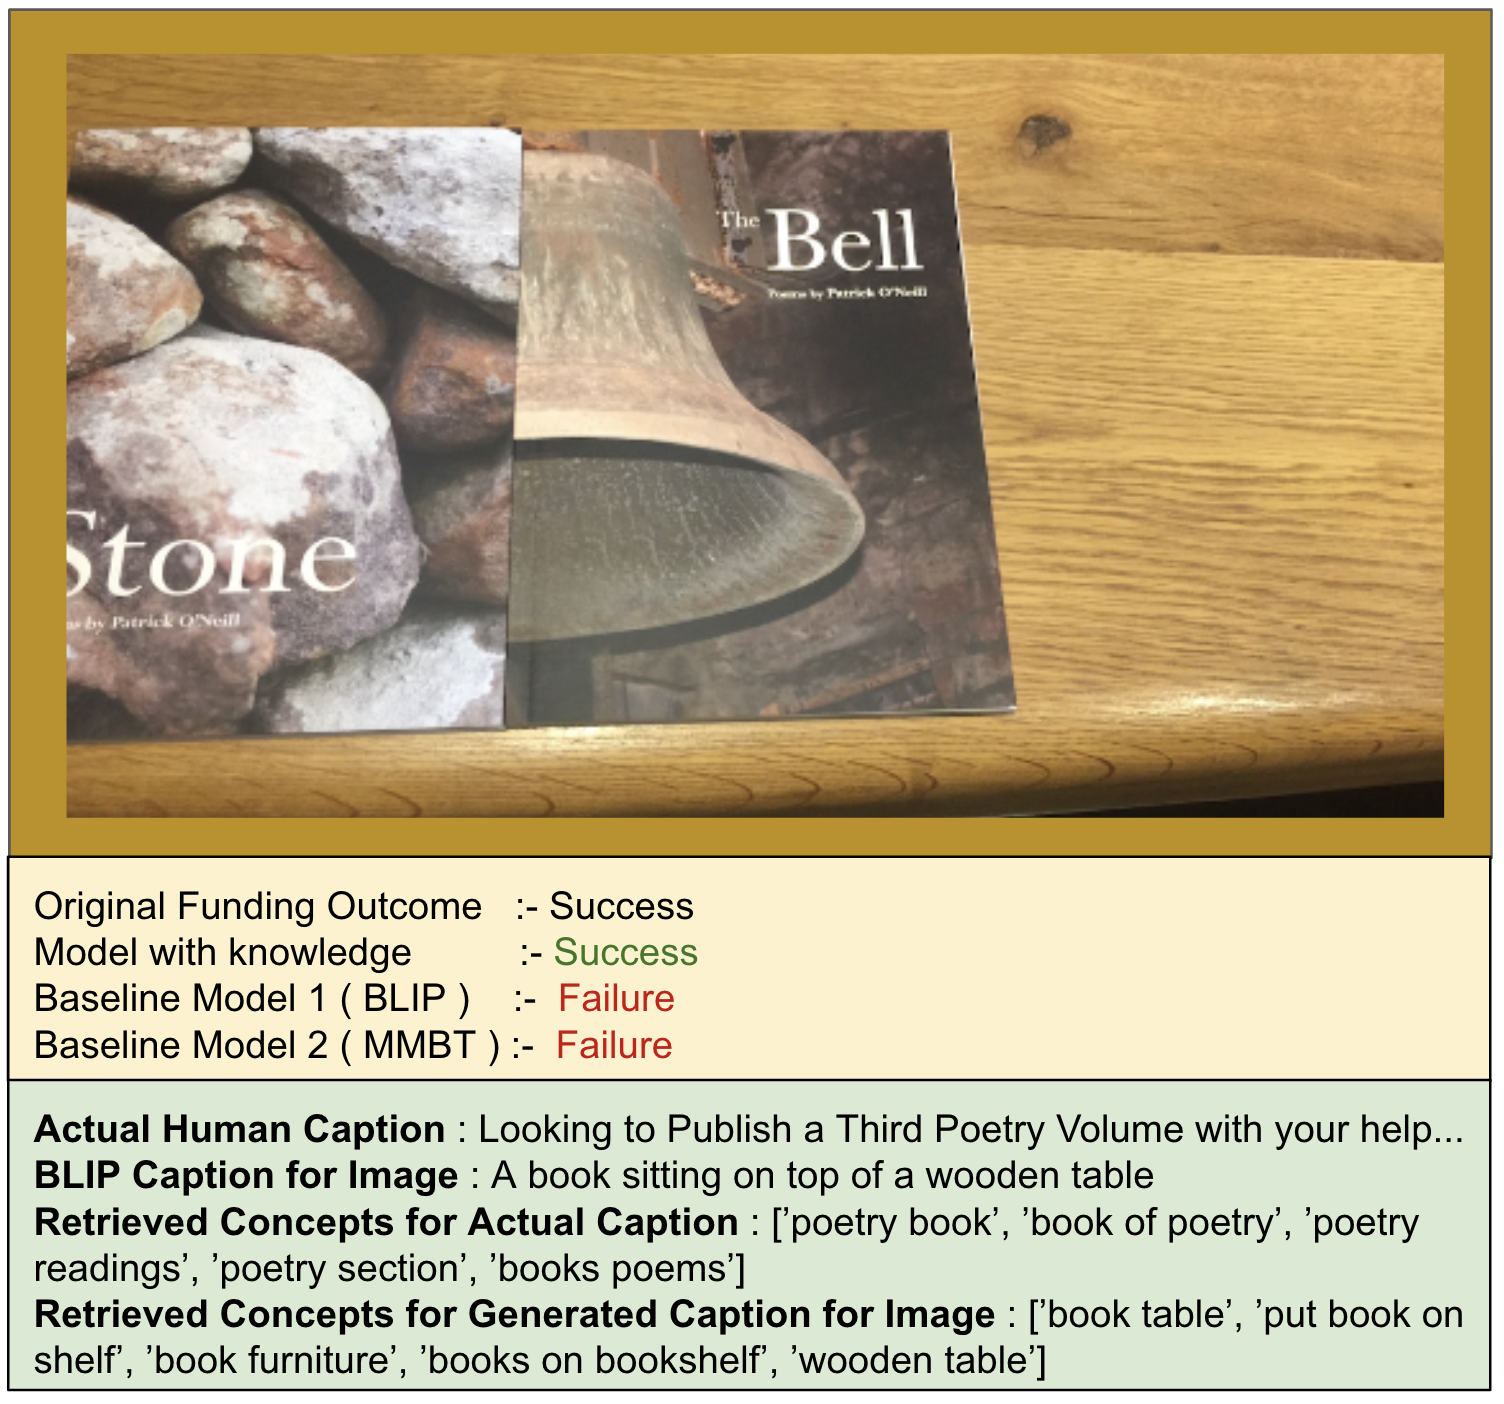
\includegraphics[width=8.5cm]{Figures/erroranalysis/error-analysis-sucess-poet.png}
% \vspace{-1em}
\caption{In the yellow box, the prediction of the model with knowledge, blip model and MMBT, In the green box, actual caption, blip caption, retrieved concepts for each modality.}
\vspace{-1.5em}
\label{fig:error-analysis-sucess-poet}
\end{figure} 

\begin{figure}[hbt!]
  \centering
  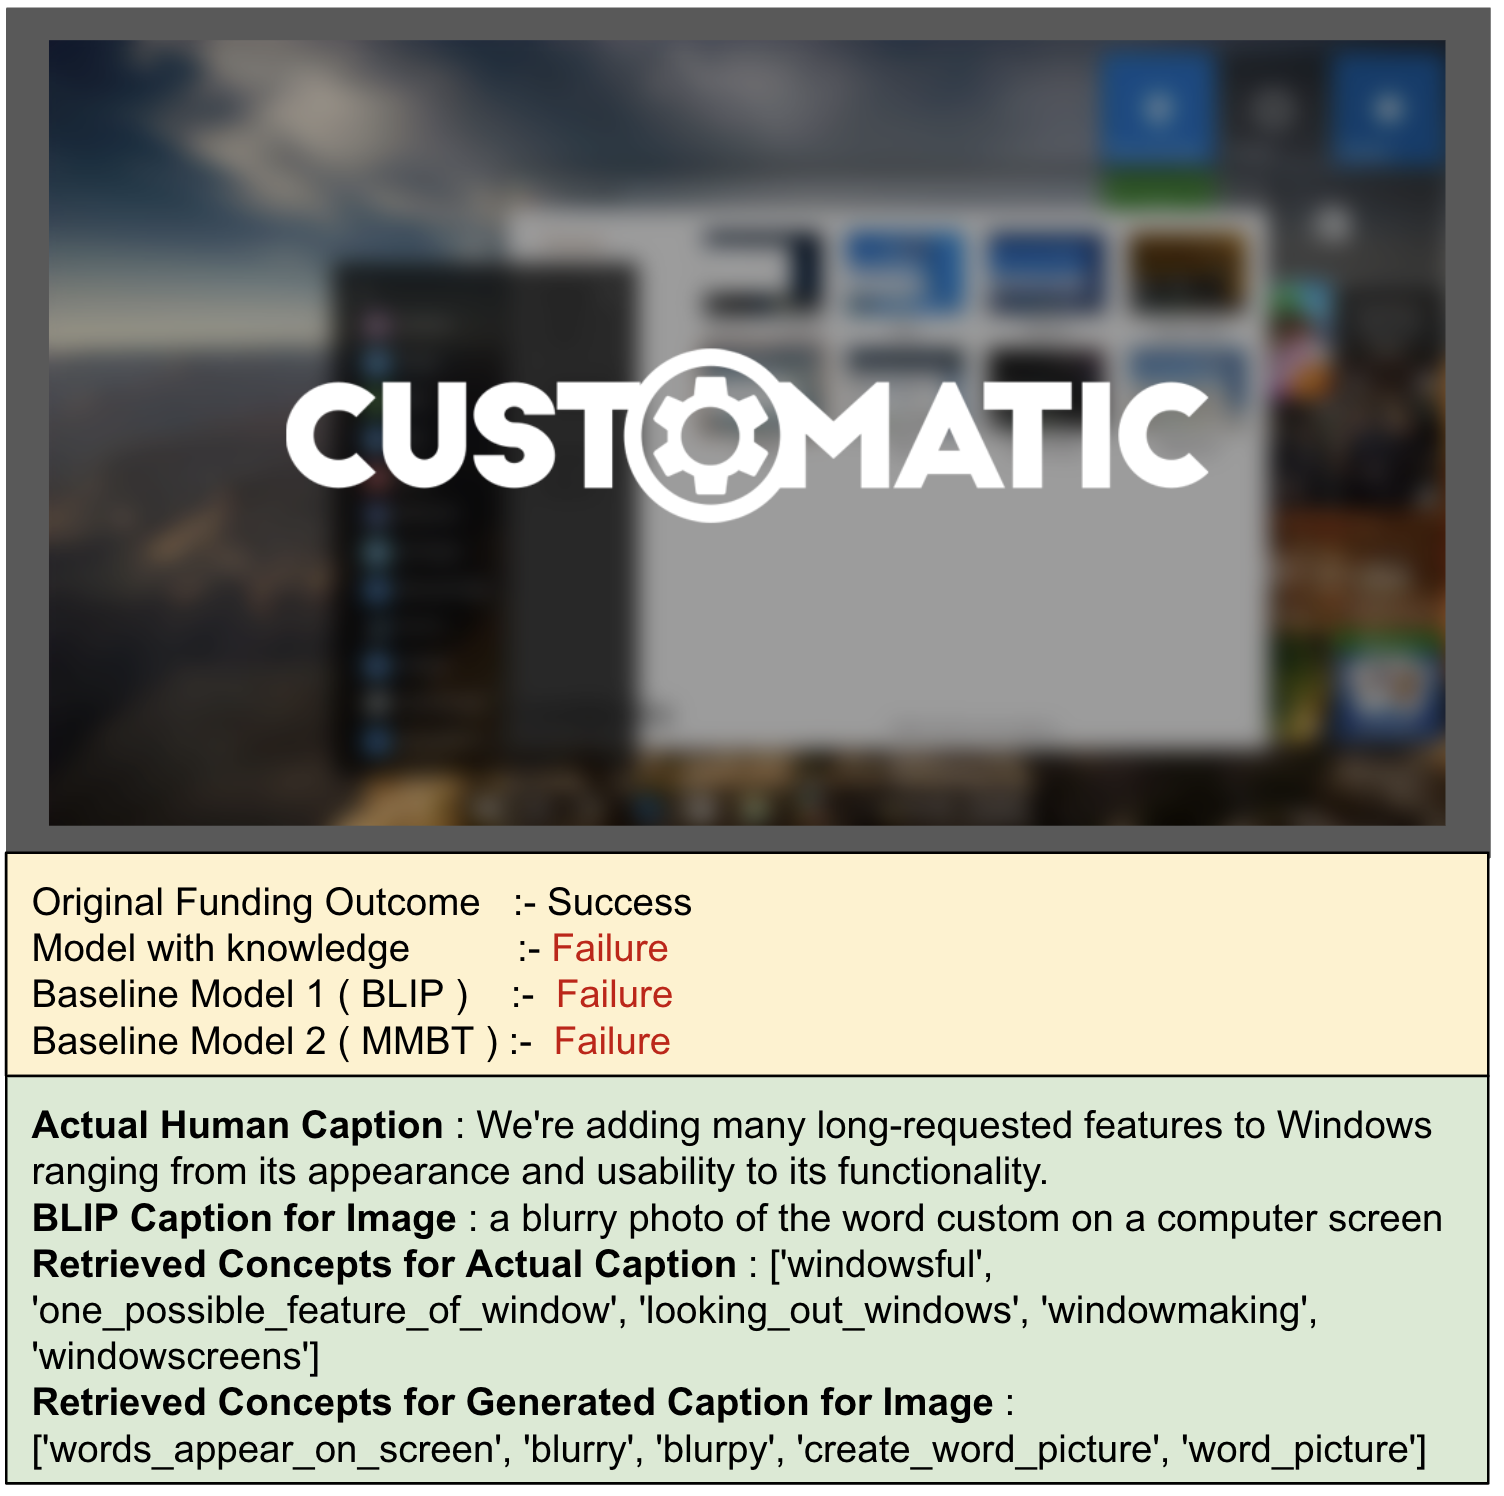
\includegraphics[width=8.5cm]{Figures/erroranalysis/error-analysis-failure-custom-windows.png}
% \vspace{-1em}
\caption{In the yellow box, the prediction of the model with knowledge, blip model and MMBT, In the green box, actual caption, blip caption, retrieved concepts for each modality. \\ 
}
\vspace{-1.5em}
\label{fig:error-analysis-failure-custom-windows}
\end{figure}

\clearpage


\section{Data Appendix}
\label{sec:dataappendix}
For our analysis, we used data from Kickstarter.com hosted on the web crawler platform Webrobots.io. We analyzed 75,810 projects that applied for Kickstarter funding in the time period between June 17, 2021, and May 19, 2022. For every project, we tracked specific project indicators such as project ID, project name, project image, the text blurb (which is taken as the text caption in our project), the current state of the project, goal amount in USD, pledged amount in USD, and industry branch.  The Pie chart below shows the project categories included art, comics, crafts, dance, design, fashion, film and video, food, journalism, music, photography, publishing, technology, and theater. Our primary outcome variable was the fundraising outcome. The data source defined four possible financ-ing outcomes: successful, canceled, failed, and live financing. Successful financing means that the project reached both its financial goal and fundraising deadline (39\% of all projects). Some 58\% of projects failed to amass the goal amount by the fundraising deadline. Five per-cent of projects were canceled prior to the fundraising campaign launch for reasons such as deadlines and/or the financial goal not being realistic. Lastly, 2\% of projects were “Live”, meaning currently in the process of fundraising. Since their final status had yet to be determined, they were excluded from the analysis. We subsumed the canceled and failed projects in the group named “unsuccessful financing”, thus effectively making fundraising outcome a dichotomous variable, i.e., successful and unsuccessful projects. Backers are individuals who pledge money to join creators in bringing projects to life,i.e., to support a cre-ative process. They receive various rewards for their engagement as a creator's way to share a piece of proj-ect with their backer community (Kickstarter, 2021). The more backers a project receives, the more chances it has to hit its goal amount and fundraising deadline. The goal amount is the amount of money creators are setting on Kickstarter.com.  For our analysis, we do not consider the number of backers, goal amount, pledged amount, pledged amount per backer, and pledged to goal ratio. According to Kick-starter.com,once a creator launches their project, the funding goal and deadline are locked in and cannot be changed. The pledged amount represents the amount of money a specific project has received from its backers. Only projects whose pledged amount hits or exceeds their goal amount within a specific deadline will be suc-cessfully financed (Kickstarter, 2021). 

\vspace{-0.5em}
\begin{figure}
  \centering
  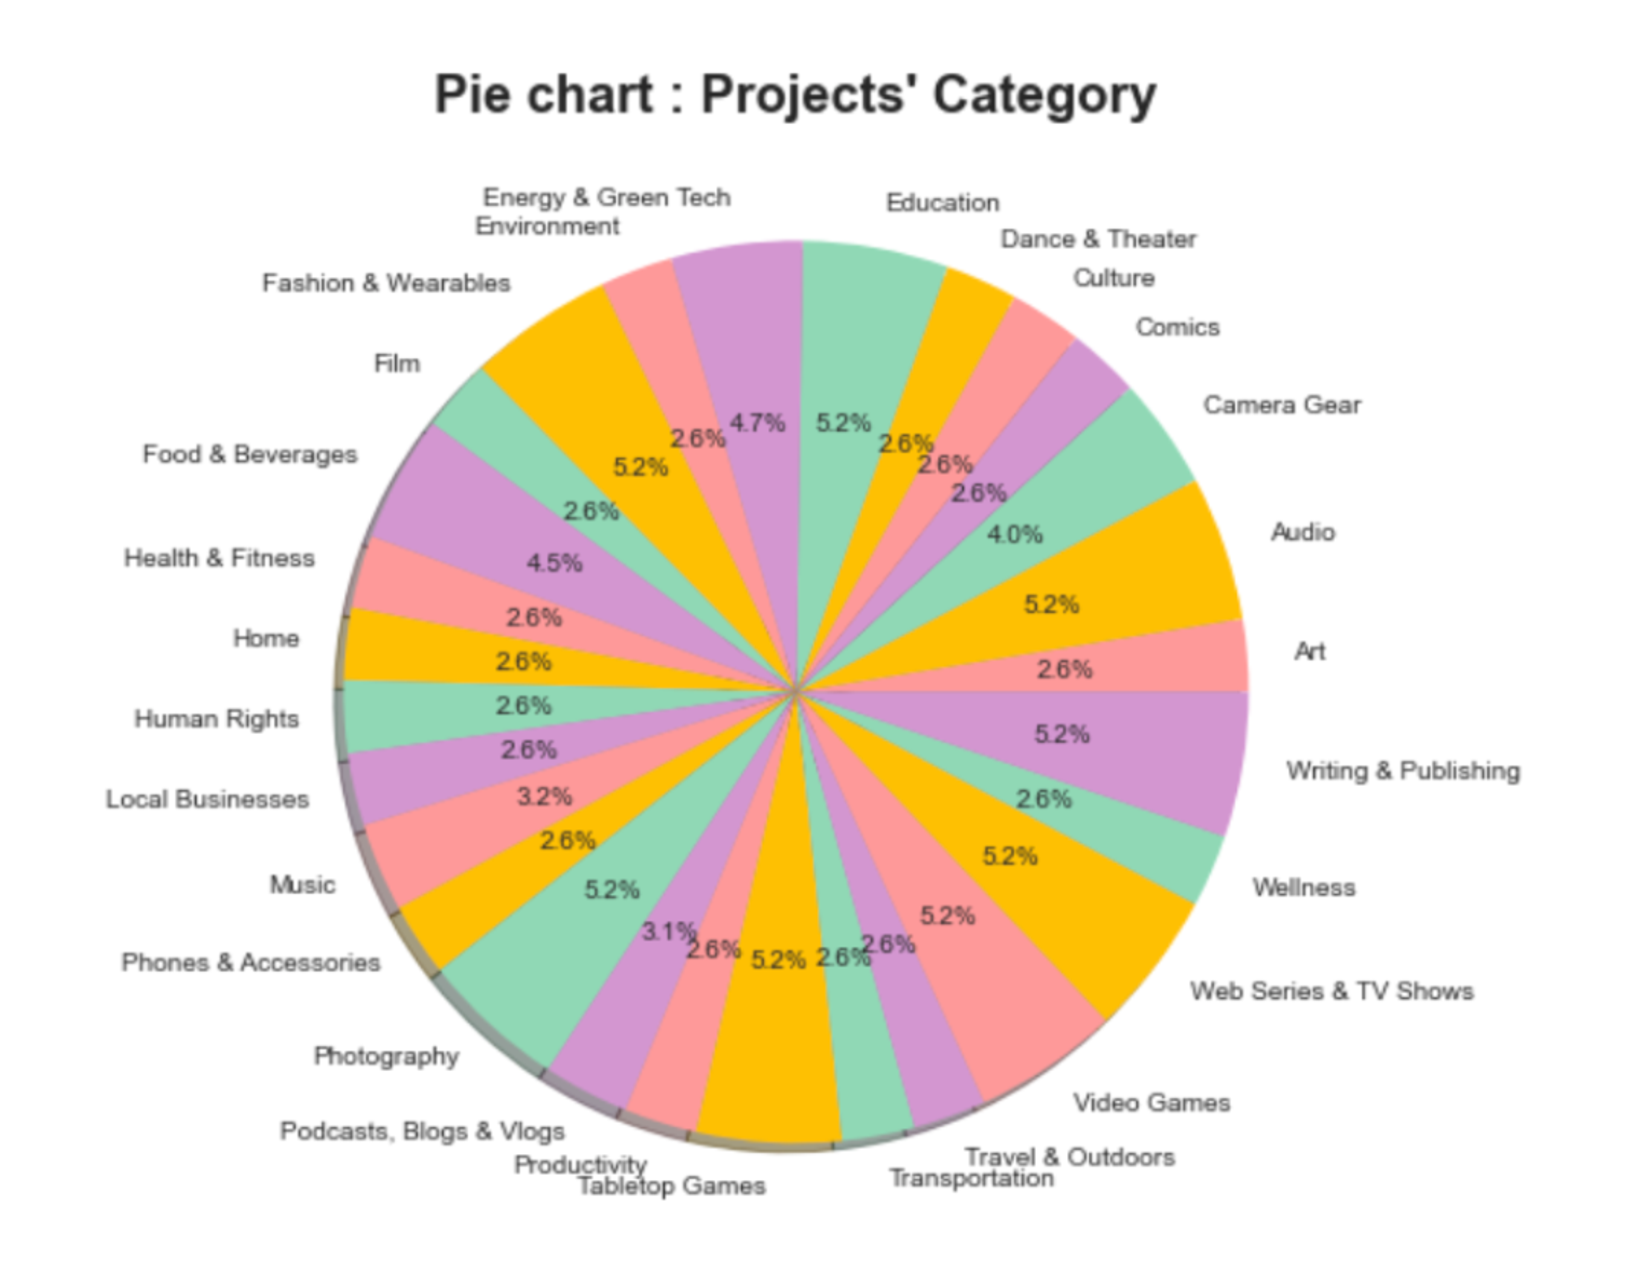
\includegraphics[width=8.5cm]{Figures/projects_pie_chart.pdf}
\vspace{-1em}
\caption{Pie chart showing type of Projects  and their percentages in Kickstarter"}
\vspace{-1em}
\label{fig:projects-pie-chart}
\end{figure} 

\clearpage

% \section{Code Appendix}
% \label{sec:codeappendix}
% \input{aaai2024/9-Codeappendix}

\newpage


% \end{document}



% Use \bibliography{yourbibfile} instead or the References section will not appear in your paper
% \nobibliography{aaai22}

% \section{Acknowledgments}

% \bigskip


\end{document}
